% !TeX encoding = UTF-8
% !TeX spellcheck = en_GB
\documentclass[12pt,letterpaper]{report}
\usepackage[utf8]{inputenc}
%\usepackage[toc,page]{appendix}
\usepackage{amsmath}
\usepackage{graphicx}
\usepackage[destlabel,pdfusetitle]{hyperref}
\usepackage{hhline} % for tabular expressions
\usepackage{multirow} % "
\usepackage{algorithmic} % code in the tabular expression explanation
\usepackage{caption}
\usepackage{subcaption} % subfigures
\usepackage{geometry} % to adjust margins
\usepackage{longtable}
\usepackage{tabu}
\usepackage{matlab-prettifier}
\lstset{style=Matlab-editor}
\usepackage{comment}
\usepackage{appendix}
\usepackage[T1]{fontenc}
\usepackage{bigfoot} % to allow verbatim in footnote
\usepackage{float}
\usepackage{xspace} % http://ctan.org/pkg/xspace (for macros)

\renewcommand{\contentsname}{Table of Contents}

\newcommand{\Appendixautorefname}{Appendix}%
\renewcommand{\chapterautorefname}{Chapter}%
\renewcommand{\sectionautorefname}{Section}%
\renewcommand{\subsectionautorefname}{Section}%
\renewcommand{\subsubsectionautorefname}{Section}%
\setcounter{secnumdepth}{3}
\newcommand\VPcomment[1]{\textcolor{red}{#1}} % Vera's comments

% abbreviations environment for acronyms
\makeatletter
\newcommand{\tocfill}{\cleaders\hbox{$\m@th \mkern\@dotsep mu . \mkern\@dotsep mu$}\hfill}
\makeatother
\newcommand{\abbrlabel}[1]{\makebox[3cm][l]{\textbf{#1}\ \tocfill}}
\newenvironment{abbreviations}{\begin{list}{}{\renewcommand{\makelabel}{\abbrlabel}%
                                              \setlength{\itemsep}{0pt}}}{\end{list}}

\newcommand{\matlab}{\mdseries\textsc{Matlab}\xspace} %mdseries for reduced 
%font weight in section headings
\newcommand{\simulink}{Simulink\xspace}
\newcommand{\mathworks}{MathWorks\xspace}

\newcommand{\tool}{Auto Layout\xspace}

%Raising \hypertarget links a line https://tex.stackexchange.com/questions/17057/hypertarget-seems-to-aim-a-line-too-low
%above does not work for tabular-like environments, replaced hypertarged with \phantomsection\label{key} as per https://tex.stackexchange.com/questions/212161/adjust-jump-location-of-hypertargets
%combined above with \raisebox as seen here https://tex.stackexchange.com/questions/54935/reference-to-a-label-linked-with-a-longtable-row
\makeatletter
\newcommand{\mylabel}[1]{\raisebox{\f@size pt}{\phantomsection}\label{#1}}
\makeatother

\newcommand{\PushDownLink}{The Data Store Push-Down Tool}
%Requirement links
\newcommand{\TestingInputsOutputsLink}{\hyperref{srs.pdf}{}{subsec:TestingInputsOutputs}{the Testing Inputs \& Outputs Requirement}}
\newcommand{\IntegrationLink}{\hyperref{srs.pdf}{}{subsec:Integration}{the Integration Requirement}}
\newcommand{\SOCReqLink}{\hyperref{srs.pdf}{}{subsec:SOC}{the SOC Requirement}}
\newcommand{\BPCMFlowchartLink}{\hyperref{srs.pdf}{}{fig:BPCMflowchart}{the BPCM Flowchart}}
\hypersetup{
  linktocpage,
  colorlinks,
  linkcolor=blue,
  urlcolor=blue,
  pdfkeywords={{AutoLayout} {documentation} {Simulink} {McMaster University}},
  pdfstartpage=2
}

\begin{document}
  
  \title{\tool: Software Design Description (Draft)}
  
  \author{
    Harjot Nijjar\\
    Curtis Milo \\
  }
  
  \maketitle
  
  \tableofcontents

\chapter{Introduction}

\par This document is a Software Design Description (SDD) for the \tool tool. The purpose of the tool is to automatically format any Simulink model to improve its visual layout, and this is accomplished by arranging the blocks and lines such that the readability of the model increases. A high level hierarchy design is presented which groups similar functions and scripts based on their functionality. Furthermore, a layout engine is used to create an initial layout and then some post-processing is done in MATLAB to refine the layout. Currently, there are two engines: Graphiz and GraphPlot. Graphiz is a third party software and it is not covered in this report, while GraphPlot is a built into MATLAB and information about it is included in this document. More specifically, the functions the \tool tool uses to interface with GraphPlot engine are included in this document. Also, this document contains functions/scripts used for the \tool tool, their functionality, and description of the their internal design. The purpose of this document is to provide a clear understanding of how the \tool tool is structured and how the various functions/scripts used in this tool relate to each other.

\par The outline of the document is as follows. Chapter~\ref{TopLevelDesign} presents an architectural view of the tool. Chapter~\ref{LayoutModules} presents the detailed design of the tool, and Chapter~\ref{GraphPlotModules} presents the modules for the MATLAB GraphPlot engine. Lastly, a list of abbreviations used in this document is included in Appendix \ref{A}.

\chapter{Top Level Design Overview} \label{TopLevelDesign}
\par The \tool tool contains many functions and it is difficult to see the relationships and similarities between the functions. Therefore, the functions that have a similar functionality, or functions that have similar applications, are grouped together as modules as shown below:
\begin{figure}[h]
	\centering
	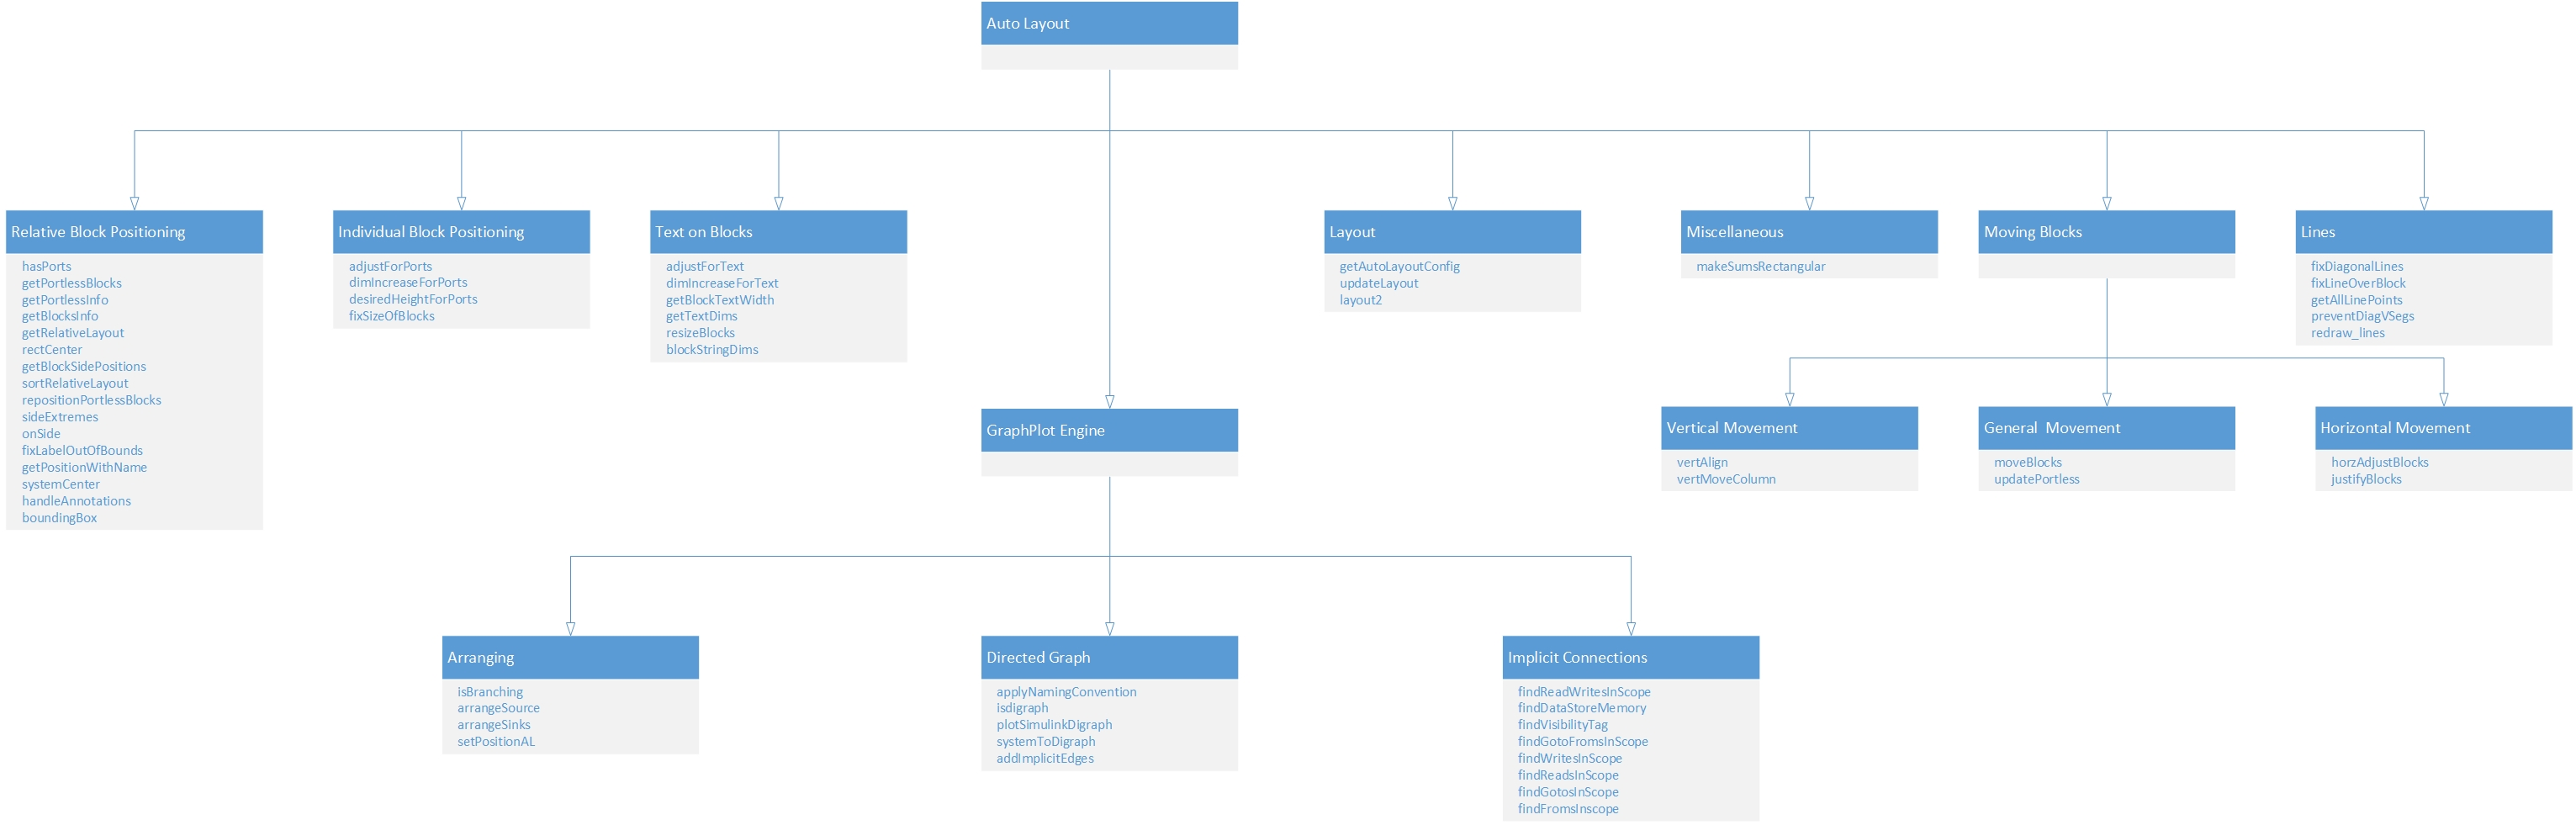
\includegraphics[width=1\linewidth]{images/AutoLayout_chart}
	\caption{\tool Tool Overview}
	\label{fig:autolayoutchart}
\end{figure}
%The picture is alittle small to view when at normal document size

\par Each block represents a module and the header of the block (blue colour) indicates the name of the module. The blocks also contain the name of the functions which belong to that module. Furthermore, a module can be sub-divided and the relationship between the parent module and the child module (sub-module) is represented by arrows, and the direction of the arrow indicates the parent-to-child relationship. Note that the functions in the parent module do not have to call functions from the child module(s). Modules are simply used to group functions based on their functionality. The GraphPlot Engine module and its child modules are functions that the \tool tool uses to interface with the MATLAB GraphPlot engine.
\par The tool consists of the following modules: Lines, Moving Blocks, Vertical Movement, Horizontal Movement, General Movement, Miscellaneous, Layout, GraphPlot Engine, Implicit Connections
\begin{itemize}
	\item Lines: Redrawing lines to avoid crossings and overlaps.
	\item Moving Blocks: Moving blocks in the layout. This module contains three sub-modules: General Movement, Horizontal Movement, and Vertical Movement. Each sub-module moves blocks in a specific direction or direction(s).
		\subitem General Movement: Move blocks in any direction.
		\subitem Vertical Movement: Only move blocks vertically
		\subitem Horizontal Movement: Only move blocks horizontally
	\item Miscellaneous: Functions that do not belong in other modules
	\item Layout: Configure the tool settings and call other functions
	\item GraphPlot Engine: Interface with the MATLAB GraphPlot engine and the model layout. This module contains three sub-modules: Implicit Connections, Directed Graph, and Arranging. Each sub-module moves interfaces with the engine for specific reasons.
		\subitem Implicit Connections: Finding implicit connections
		\subitem Directed Graph: Creating and modifying the directed graph created through GraphPlot
		\subitem Arranging: Re-arranging the nodes
	\item Text on Blocks: Determining new block sizes based on the text on a block.
	\item Individual Block Positioning: Determine new block positions and sizes based on a block's parameters
	\item Relative Block Positioning: Determine new block positions based on its current location and its surroundings
\end{itemize}

\section{Task Diagram}
\par The following shows the structure of the function calls within the main function of the auto layout tool. First the tool fetches its configuration settings. Information of the blocks is then gathered, determining which blocks are portless and then making sure Sum blocks are rectangular. Depending then on which version of Matlab or Graphical plotting preference, Graphviz/GraphPlot will determine the initial organization of the layout. From this, we get information of the blocks, and update the block positions by getting there relative layouts. Then all the blocks are resized, block positions updated again and blocks are aligned with blocks they connect to without disrupting other features of the layout. Depending on the inport/outport rules, blocks are then moved to the edges. Any portless blocks are then re-positioned and then finally any annotations are moved and shown block names are placed on the bottom of blocks.



\begin{figure}[h]
	\centering
	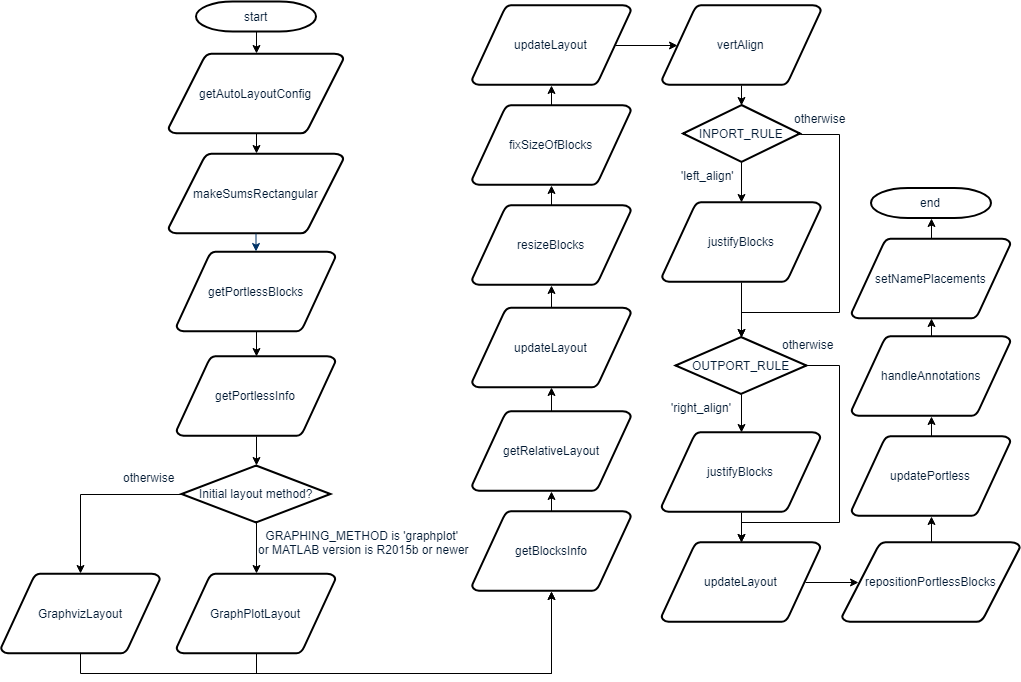
\includegraphics[width=1\linewidth]{images/AutoLayout_DrawIO_TaskDiagram}
	\caption{Auto Layout Tool Overview}
	\label{fig:taskdiagram}
\end{figure}

\section{Call Graph}

\par The \tool tool first fetches the configuration settings for tool, which are used to determine how the blocks will be organized in the layout. Then, getPortlessBlocks function is called to create a list of portless blocks and getPortlessInfo determines where to place the portless block. Then, the GraphPlot functions are called to provide an initial layout of the nodes and edges in the model. Then, a layout grid struct is created by constructing a list of blocks in the layout with ports by calling the function getBlocksInfo and getRelativeLayout. Next, appropriate block sizes are determined by calling the function resizeBlocks and fixSizeOfBlocks. Then, the vertical alignment of the blocks and lines are changed by the functions vertAlign, layout2, and justifyBlocks. Lastly, the portless blocks are moved to the appropriate edge of the layout by calling the function repositionPortlessBlocks and updatePortless.
%For this section, when referring to the initial layout. it would be good to explain what this means. Does this refer to an inital pass of the model through Graphplot tool or is this referring to the inital model positions.
\par The call graph for the tool is generated by opening up the Simulink Project created for the tool. The name of the project file is \textbf{AutoLayout\_Project.prj} and it is found in the \textbf{Simulink\textbackslash Tools\textbackslash AutoLayout} directory. The call graph is generated by running a dependency analysis. Remove/add files to the Simulink Project to remove/include files in the call graph. More information on how to run a dependency analysis for Simulink Projects can be found here:  \url{https://www.mathworks.com/help/simulink/ug/run-dependency-analysis.html}.
% LAYOUT
% *******************************************************************
\chapter{The \tool Tool: Detailed Design} \label{LayoutModules}
\section{Introduction}
 This chapter presents detailed design for each of the modules from Chapter~\ref{TopLevelDesign}, including black-box specification and detailed design of the belonging functions.
 \par The function AutoLayout is the top-level function for the \tool tool. There are several modules that \tool is organized into as stated in~\ref{TopLevelDesign}. The modules are: Layout, GraphPlot Engine, Relative Block Positioning, Individual Block Positioning, Text on Blocks, Moving Blocks, Lines and Miscellaneous. The Moving Blocks module contains three child modules: General Movement, Vertical Movement and Horizontal Movement.

\section{Layout}
\par This module is responsible for configuring the tool settings and updating the layout. The functions in this module are:
\begin{itemize}
	\item getAutoLayoutConfig
	\item updateLayout
	\item layout2
\end{itemize}
%It might be worth taking the inormation from these comments/function definitions and
%putting it into a table format. Matlab does have special comment abilities that you can use to generate an MIS from the comments.
\subsection{getAutoLayoutConfig}
\begin{lstlisting}
function val = getAutoLayoutConfig(parameter, default)
% GETAUTOLAYOUTCONFIG Get a parameter from the tool configuration file.
%
%   Inputs:
%       parameter   Configuration parameter to retrieve value for.
%       default     Value to use if parameter is not found.
%
%   Outputs:
%       val         Char configuration value.
\end{lstlisting}
\paragraph{Internal Design:} Parse the config file and search for the line that contains the string "parameter:" to determine the value of the parameter. If no parameter value is found, then the default value specified by the input is used for the tool.

\subsection{updateLayout}
\begin{lstlisting}
function updateLayout(address, layout)
% UPDATELAYOUT Move blocks to their new positions designated by layout.
%
%   Inputs:
%       address         Simulink system name or path.
%       layout          As returned by getRelativeLayout.
%
%   Outputs:
%       N/A
\end{lstlisting}
\paragraph{Internal Design:} The blocks positions in the layout are updated by calling the function \hyperref[moveBlocks]{moveBlocks}.
%What is the modivation of having update layout if it is used to call moveBlocks. Does this function alse find every simulink element and call moveBlocks on each?
\subsection{layout2}
\begin{lstlisting}
function layout = layout2(address, layout, systemBlocks)
% LAYOUT2 Performs a series of operations to further improve the layout
% from AutoLayout. The functionality it provides is listed below roughly 
% ordered with when it is done in this function.
%   Moves inputs and outputs to the outsides when it is easy (and not messy) to do so
%   Adjusts the vertical spacing between close blocks
%   Keeps labels on screen if they went off to the left
%   Expands small blocks by extending their right side
%   Adjusts spacing between blocks horizontally to be more reasonable
%   Redraws lines,
%       first uses the same method as in initLayout,
%       then prevents/removes diagonal lines,
%       then fixes a case where the autorouting isn't very good,
%       then fixes lines going over blocks,
%       and then fixes overlapping between vertical segments of lines
%   Places blocks with no ports (such as Data Store Memory blocks) along the top or bottom of the system horizontally
%       It chooses which half the system to place the block in based on the half it started in
%
%   Inputs:
%       address         Simulink system name or path.
%       systemBlocks    List of blocks in address.
%
%   Updates:
%       layout          Input in the same format as returned by 
%                       getRelativeLayout. Returned according to the
%                       operations performed in this function.
\end{lstlisting}
\paragraph{Internal Design:} This function calls other functions that deal with the lines in the layout.

%This one in particular is hard for the user to read.
%For this line: " Moves inputs and outputs to the outsides when it is easy (and not messy) to do so". It might be worth going into detail on when and when you cannot move inputs and outputs.

\section{GraphPlot Engine}
\par Refer to Chapter~\ref{GraphPlotModules}. The GraphPlot does preprocessing for the layout, and this engine can be replaced by another engine. So, it documented in another chapter because the GraphPlot section deals with functions that interface with the MATLAB GraphPlot engine, and  because the engine can be replaced by another one. Also, the Graphplot portion of the tool is distinct from the rest of the \tool code.

%MOVING BLOCKS ***********************************************************************************************************************************************
\section{Moving Blocks}
\par This module is responsible for movement of the blocks in the layout. This module contains three sub-modules which are:
\begin{itemize}
	\item \hyperlink{General Movement}{General Movement}
	\item Vertical Movement
	\item Horizontal Movement
\end{itemize}

\subsection{General Movement} \label{General Movement}
\par This module is responsible for moving blocks in any direction. The functions in this module are:
\begin{itemize}
	\item moveBlocks
	\item updatePortless
\end{itemize}

\subsubsection{moveBlocks} \label{moveBlocks}
\begin{lstlisting}
function moveBlocks(address, blocks, positions)
% MOVEBLOCKS Move blocks in address to the given positions.
%
%   Inputs:
%       address     Simulink system name or path.
%       blocks      Cell array of full block names.
%       positions   Cell array of positions corresponding with blocks (i.e.
%                   blocks{i} should be moved to positions{i}; blocks and
%                   positions are of the same length).
%                   Each value should be in a vector as returned by
%                   get_param(gcb, 'Position').
%
%   Outputs:
%       N/A
%
%   Example:
%       moveBlocks('AutoLayoutDemo',{'AutoLayoutDemo/In1', ...
%           'AutoLayoutDemo/In2'}, {[-35,50,-15,70],[-35,185,-15,205]})
\end{lstlisting}
\paragraph{Internal Design:} Move the blocks and ports in the layout to the new position defined in the layout grid by editing their position parameter values. Also, the signal lines in the layout are redrawn by calling the function \hyperref[redraw_lines]{redraw\_lines}.

\subsubsection{updatePortless} \label{updatePortless}
\begin{lstlisting}
function updatePortless(address, portlessInfo)
% UPDATEPORTLESS Move blocks to their new positions designated by portlessInfo.
%
%   Inputs:
%       address         Simulink system name or path.
%       portlessInfo    As returned by getPortlessInfo.
%
%   Outputs:
%       N/A
\end{lstlisting}
\paragraph{Internal Design:} Only move portless blocks by obtaining the name and new desired positions of the blocks using portlessInfo. The blocks are then moved by calling the function \hyperref[moveBlocks]{moveBlocks}.

%It is usally best practice to try and not mention where the data is being recieved from. An alternative would be: "Moves the blocks to the new positions based on the information provided on the portless blocks"

\subsection{Horizontal Movement} \label{Horizontal_Movement}
\par This module is responsible for moving blocks in horizontally. The functions in this module are:
\begin{itemize}
	\item horzAdjustBlocks
	\item justifyBlocks
\end{itemize}

\subsubsection{horzAdjustBlocks}  \label{horzAdjustBlocks}
\begin{lstlisting}
function layout = horzAdjustBlocks(layout, col, x)
% HORZADJUSTBLOCKS Horizontally move blocks in the layout, to the right of
%   the column, right by x.
%
%   Inputs:
%       layout          As returned by getRelativeLayout.
%       col             Column number, to the left of which blocks will not be moved.
%       x               Number of pixels to move blocks.
%
%   Outputs:
%       layout      With modified (left, right) position information.
\end{lstlisting}
\paragraph{Internal Design:} Change the left and right position values of all blocks and ports equally that are to the right of the specified column. This is done by incrementing the positions by the desired change in the horizontal position of all blocks in each column after the specified column.

\subsubsection{justifyBlocks}
\begin{lstlisting}
function layout = justifyBlocks(address, layout, blocks, justifyType)
% JUSTIFYBLOCKS Align blocks to facilitate the use of straight lines in
%   connections by repositioning blocks vertically.
%   Currently only attempts to align blocks which connect to a single block
%   through an in/outport.
%
%   Inputs:
%       address         Simulink system name or path.
%       layout          As returned by getRelativeLayout.
%       blocks          List of blocks to be affected by the justification.
%       justifyType     How the blocks will be aligned: left justified (1) or
%                       right justified (3) (The numbers correspond with
%                       the position parameter of blocks i.e. a block with
%                       position [1 2 3 4] has a left position 1 and a
%                       right position of 3).
%
%   Output:
%       layout          With modified position information.
%
% Pushes blocks either too far right or left.
% If doing so would cause line crossings then affected blocks won't be moved.
\end{lstlisting}
\paragraph{Internal Design:} This function either takes in a list of inports or outports and moves inports and outports to the left and right edges of the layout respectively. For inports, the first column is ignored for justification, and for outports, the last column is ignored for justification (ports are already justified). For each port, check if it suitable for justification by checking what column it is in. If the port is suitable for justification, check if there are any blocks or lines in the way. If there are no blocks or lines in the way, the port is moved to the first or last column in the layout grid (depending on the justification). Blocks are determined to be in the way if there are no overlapping blocks in the columns that the port needs to across over or into, and this is done by comparing the top and bottom positions of the port and the blocks in the columns of interest. Lines are determined to be in the way by first finding all lines in the layout. Then, the difference between middle x position of the port's current location and desired justified position is calculated. This is accomplished by taking the midpoint x position value of the first block in the column that the port is being justified into. Next, for each line's segment, check if the port is between the starting and ending y position of the line segment. If so, check if the imaginary line between the desired justified location of the port and the current position of the port lies between the starting and ending x position of the line segment. If so, then a line is in the way of the justification of the port. Note that the imaginary line is constructed by taking two points. The first point is the current side position of interest for the port (left or right side). The second point is the side plus the difference between the midpoint of the port and the midpoint of the first block in the column the port should be moved into.

\subsection{Vertical Movement} \label{Vertical_Movement}
\par This module is responsible for moving blocks in vertically. The functions in this module are:
\begin{itemize}
	\item vertMoveColumn
	\item vertAlign
\end{itemize}

\subsubsection{vertMoveColumn}
\begin{lstlisting}
function layout = vertMoveColumn(layout, row, col, y)
% VERTMOVECOLUMN Vertically move blocks in col and below row in layout.grid
%   downward by y.
%
%   Inputs:
%       layout      As returned by getRelativeLayout.
%       row         Row number, below which blocks will be moved.
%       col         Column number, in whihch blocks will be moved.
%       y           Number of pixels to move blocks.
%
%   Outputs:
%       layout      With modified position information.
\end{lstlisting}
\paragraph{Internal Design:} Move blocks vertically that are in the specified column and below the specified row. This is done by changing the top and bottom position values of all blocks and ports equally.

\subsubsection{vertAlign}
\begin{lstlisting}
function layout = vertAlign(layout)
% VERTALIGN Align blocks to facilitate the use of straight lines in connections
%   by repositioning blocks vertically. Currently only attempts to align blocks
%   which connect to a single block through an inport/outport.
%
%   Inputs:
%       layout          As returned by getRelativeLayout.
%
%   Outputs:
%       layout          With modified position information.
\end{lstlisting}
\paragraph{Internal Design:} First, a list of suitable blocks to vertically align is created. The criteria for aligning a block is that it must have only one port in total and if it has an outport, the block must not be connected to more than one block. Then in a while loop, go through the list previously created, starting with the last block first and ending at the first block. For each block, an anchor block is used to help vertically align the block. If the block has one outport, then its destination block is used as an anchor, and if the block has one inport, then its source block is used as an anchor. The anchor is then used to calculate how much the block needs to be moved to be aligned with the anchor. Then, it is determined whether or not the block has sufficient room to move based on its current location in the layout. If there is enough room to move the block, it is moved to the desired location and it is removed from the list of blocks that needs to be vertically aligned. If at least one block was vertically aligned, then the while loop continues and loops through the list of blocks to vertically align again to check if some blocks that could not be aligned before can be aligned now. If no blocks can be vertically aligned, the while loop is exited.

% RELATIVEBLOCK POSITIONING *************************************************************************************************************************************
\section{Relative Block Positioning}
\par This module is responsible for the calculating new block position values based on the relative location in the layout. The functions in this module are:
\begin{itemize}
	\item hasPorts
	\item getPortlessBlocks
	\item getPortlessInfo
	\item getBlocksInfo
	\item getRelativeLayout
	\item rectCenter
	\item getBlockSidePositions
	\item sortRelativeLayout
	\item repositionPortlessBlocks
	\item sideExtremes
	\item onSide
	\item fixLabelOutOfBounds
	\item getPositionWithName
	\item systemCenter
	\item handleAnnotations
	\item boundingBox
\end{itemize}

\subsection{hasPorts} \label{hasPorts}
\begin{lstlisting}
function hasPorts = hasPorts(block)
% HASPORTS Check if a block has any ports.
%
%   Inputs:
%       block       Full name of a block. If a cell array is given, the first
%                   element is used.
%
%   Outputs:
%       hasPorts    Whether the block has one or more ports (1), or none (0).
\end{lstlisting}
\paragraph{Internal Design:} A block has no ports if it is not connected to any other blocks in the layout.

\subsection{getPortlessBlocks}
\begin{lstlisting}
function portlessBlocks = getPortlessBlocks(blocks)
% GETPORTLESSBLOCKS Find blocks that have no ports from a list of blocks.
%
%   Inputs:
%       blocks          Cell array of block names.
%
%   Outputs:
%       portlessBlocks  Cell array of block names with no ports.
\end{lstlisting}
\paragraph{Internal Design:} Constructs a list of all portless blocks in the layout by calling the function \hyperref[hasPorts]{hasPorts} for each block in the layout.

\subsection{getPortlessInfo}
\begin{lstlisting}
function [portlessInfo, smallOrLargeHalf] = getPortlessInfo(portless_rule, systemBlocks, portlessBlocks)
% GETPORTLESSINFO Find the name and position about the portless blocks. For
%   position, also check which half of the system each block is in, relative
%   to the others (checks top/bottom vs. left/right half based on relevance
%   with portless_rule).
%
%   Inports:
%       portless_rule   Rule by which portless blocks should later be
%                       positioned. See PORTLESS_RULE in config.txt.
%       systemBlocks    List of all blocks in a system.
%       portlesBlocks   List of portless blocks in a system.
%
%   Outports:
%       portlessInfo        Struct of portless blocks' fullname and position.
%       smallOrLargeHalf    Map relating blocks with the side of the system
%                           they should be placed on.
\end{lstlisting}
\paragraph{Internal Design:} Create a list of the struct that contains the name and current position of all portless blocks in the layout.

\subsection{getBlocksInfo}
\begin{lstlisting}
function blocksInfo = getBlocksInfo(sys)
% GETBLOCKSINFO Get a struct with name and position information of all blocks
%   in a system.
%
%   Input:
%       sys     System address for which to get blocksInfo.
%
%   Outputs:
%       blocksInfo              Struct of data representing current block data.
%       blocksInfo(i).fullname  Fullname of a block.
%       blocksInfo(i).position  Position of a block.
\end{lstlisting}
\paragraph{Internal Design:} Create a list of the struct that contains the name and current position of all blocks and ports in the layout. All blocks and ports are found in the layout by searching for blocks and ports in the current layout.

\subsection{getRelativeLayout}
\begin{lstlisting}
function [layout] = getRelativeLayout(blocksInfo)
% GETRELATIVELAYOUT Find the relative layout of the blocks within a grid.
%
%   Inputs:
%       blocksInfo  As returned by getLayout.
%
%   Outputs:
%       layout      Struct describing the layout of blocks in blocks info.
%                   layout.grid is organized such that all blocks with the
%                   same j in layout.grid{i,j} have the same x coordinate at
%                   their centre, and such that the top position decreases with
%                   increase in i.
%                   layout.colLengths is created such that
%                   layout.colLengths{j} is the number of blocks in the
%                   grid with that j value (i.e. number of blocks in that
%                   column).
%                   The maximum j for layout.grid{i,j} is size(layout.grid,2).
%                   If (i <= colLengths(j)) then a block will be returned.
%                   If (colLengths(j) < i <= size(layout.grid,1)) then [] will be returned.
\end{lstlisting}
\paragraph{Internal Design:} Create a layout grid of all the blocks/ports in the layout. First of all, the column number each block belongs to is determined by comparing the block's centre x position value to a sorted unique list of all blocks' centre x positions. Secondly, the current number of blocks in each column is kept track of in a list. The layout grid struct contains the blocks in each column and the number of blocks in each column. Lastly, the layout grid is sorted by calling the function \hyperref[sortRelativeLayout]{sortRelativeLayout}.

\subsection{rectCenter}
\begin{lstlisting}
function [x,y] = rectCenter(positions)
% RECTCENTER Find the coordinates of the center of a rectangle.
%
%   Inputs:
%       positions   Cell array of vectors of coordinates in the form
%                   [left top right bottom].
%
%   Outputs:
%       x           Cell array of x coordinates of the rectangle centers.
%       y           Cell array of y coordinates of the rectangle centers.
\end{lstlisting}
\paragraph{Internal Design:} Determine the centre by calculating the average position of the top and bottom position and the left and right position.

\subsection{getBlockSidePositions} \label{getBlockSidePositions}
\begin{lstlisting}
function sidePositions = getBlockSidePositions(blocks, side)
% GETBLOCKSIDEPOSITIONS Find the *unique* block positions for a given side
%   of a set of blocks.
%
%   Inputs:
%       blocks          Cell array of the full names of block(s).
%                       If a cell array is given for one of the block names,
%                       the first element is used.
%
%       side            Number respesenting the following:
%                           1 - Left
%                           2 - Top
%                           3 - Right
%                           4 - Bottom
%                           5 - Midpoint between results of 1 and 3
%                           6 - Midpoint between results of 2 and 4
%
%   Outputs:
%       sidePositions   Vector of unique doubles for the positions.
\end{lstlisting}
\paragraph{Internal Design:} Determine the specific side positions of list of blocks by obtaining it from the blocks' position parameter values. If the centre x or y positions of the block is requested, an average of the two points of interest are calculated to determine the side position values.

\subsection{sortRelativeLayout} \label{sortRelativeLayout}
\begin{lstlisting}
function grid = sortRelativeLayout(grid, colLengths)
% SORTRELATIVELAYOUT Sort blocks in grid within columns by their top positions.
%
%   Inputs:
%       grid        Format as defined in getRelativeLayout.
%       colLengths  Format as defined in getRelativeLayout.
%
%   Outputs:
%       grid        Same format, but sorted so that layout is accurate for
%                   relative vertical positions.
\end{lstlisting}
\paragraph{Internal Design:} Sort each column individually by the vertical position of the blocks in the columns in descending order (i.e., the first block in a row is at the highest position for the column it is in). For each column, the vertical positions of the blocks is converted into a vector and a MATLAB function is used to determine the order of indexes for the vector to sort it. Then, the grid is edited and sorted based on the ordered indexes. Since not all columns contain the same number of blocks, extra row entries for a column are left empty.

\subsection{repositionPortlessBlocks}
\begin{lstlisting}
function portlessInfo = repositionPortlessBlocks(portlessInfo, layout, portless_rule, smallOrLargeHalf, sort_portless)
% REPOSITIONPORTLESSBLOCKS Reposition portless blocks to a side of the system.
%   Organize portless blocks into groups on the designated sides.
%
%   Inputs:
%       portlessInfo        As returned by getPortlessInfo.
%       layout              As returned by getRelativeLayout.
%       portless_rule       Rule by which portless blocks should be
%                           positioned. See PORTLESS_RULE in config.txt.
%       smallOrLargeHalf    Map relating blocks with the side of the system
%                           they should be placed on.
%       sort_portless       Determines how to sort the portless blocks
%                           after the side is determined. See SORT_PORTLESS
%                           in config.txt.
%
%   Outputs:
%       portlessInfo        Updated portlessInfo with new positions.
\end{lstlisting}
\paragraph{Internal Design:} Portless blocks are placed in a specific side of the layout and sorted based on the tool configuration settings. The portless blocks are spaced evenly by an arbitrary amount.

\subsection{sideExtremes}
\begin{lstlisting}
function [leftBound, topBound, rightBound, botBound] = sideExtremes(layout, portlessInfo, ignorePortlessBlocks)
% SIDEEXTREMES Find the extreme positions (left, top, right, and bottom)
%   among blocks in layout and portlessInfo (unless portless blocks
%   shouldn't be considered).
%
%   Inputs:
%       layout                  As returned by getRelativeLayout.
%       portlessInfo            As returned by getPortlessInfo.
%       ignorePortlessBlocks    Whether to consider portlessInfo (1) or not (0).
%
%   Outputs:
%       leftBound               Left bound of blocks of interest.
%       topBound                Top bound of blocks of interest.
%       rightBound              Right bound of blocks of interest.
%       botBound                Bottom bound of blocks of interest.
\end{lstlisting}
\paragraph{Internal Design:} Extreme bound values are used as the default bounding positions of the layout. If portless blocks are being ignored for the maximum bounds, then the new bounding locations are found by looping through each block in the layout grid and comparing the block's position to the current bounds. If the block lies outside of the current bounds, then its position values are used to update the current bounds. If portless blocks are not being ignored, the current bounds are then compared to the position of the portless blocks to determine the bounds.

\subsection{onSide}
\begin{lstlisting}
function bool = onSide(block, center, side)
% ONSIDE Determine whether or not the center of block is on a particular side of
%   the system.
%
%   Inputs:
%       block   Full block name.
%       center  Center of the system for the given side (e.g. if side is
%               'left', center will be halfway between the largest and
%               smallest X positions of blocks in the system).
%       side    Either 'left' or 'top'. Indicates the side to compare
%               the given block's center with. E.g. If side is 'left', the
%               function checks if the center of the block is on the left
%               half of the system (if it's a tie then choose left)
%
%   Outputs:
%       bool    Whether or not the given block is on the indicated side of the system.
\end{lstlisting}
\paragraph{Internal Design:} The block's position is compared to the centre of the layout. Either centre x or y position is compared with the midpoint x or y position of the block respectively. The block's midpoint position is determined by calling the function \hyperlink{getBlockSidePositions}{getBlockSidePositions}. 

\subsection{fixLabelOutOfBounds}
\begin{lstlisting}
function layout = fixLabelOutOfBounds(layout)
% FIXLABELOUTOFBOUNDS Horizontally move blocks in the layout away from the
%   system's left bound if a block's name label extends past it.
%
%   Inputs:
%       layout  As returned by getRelativeLayout.
%
%   Outputs:
%       layout  With modified (left, right) position information for labels.
\end{lstlisting}
\paragraph{Internal Design:} For each column, go through all of the blocks in the column and determine greatest difference between a blocks name's width and the block's width. All blocks in the column and all blocks to the right of the column are moved horizontally by the greatest difference divided by two by calling the function \hyperlink{horzAdjustBlocks}{horzAdjustBlocks}. Nothing is done if no block's name is wider than its width in a column.

\subsection{getPositionWithName}
\begin{lstlisting}
function bounds = getPositionWithName(block)
% GETPOSITIONWITHNAME Find the bounding box of a block accounting for where
%   its name appears if showing. Does not currently account for other block
%   parameters that might be showing.
%
%   Inputs:
%       block   SSimulink block name or handle.
%
%   Outputs:
%       bounds  Bounding box of the block. Returned in the format
%               [left, top, right, bottom].
\end{lstlisting}
\paragraph{Internal Design:} The size of the text for the block's/port's name is calculated by calling the function \hyperlink{blockStringDims}{blockStringDims}. The width of the name is compared to the block's/port's bounds. If the width of the name is the greater of the two, half of the different between name's width and the block's width is added to the right bound and subtracted from the left bound. Then, depending on where the name is placed (below or above the block), it is added to the bottom or top bounds of the block/port.

\subsection{systemCenter}
\begin{lstlisting}
function [x,y] = systemCenter(blocks)
% SYSTEMCENTER Find the center of the system (relative to the block positions).
%
%   Inputs:
%       blocks  List of blocks.
%
%   Outputs:
%       x       x coordinate of the center of the bounds of the blocks.
%       y       y coordinate of the center of the bounds of the blocks.
\end{lstlisting}
\paragraph{Internal Design:} The centre of the layout is calculated by taking the average of the bounds of the layout in the x and y directions. The bounds of the layout are determined by first setting extreme values and then by going through every block and seeing if the block is outside of the current bound. If so, then the current bounds are updated to include the block.

\subsection{handleAnnotations}
\begin{lstlisting}
function handleAnnotations(layout, portlessInfo, annotations, note_rule)
% HANDLEANNOTATIONS Move portless blocks to the right side of the system.
%   The annotations should not extend too far below the bottom of the
%   system.
%
%   Inputs:
%       layout          As returned by getRelativeLayout.
%       portlessInfo    As returned by getPortlessInfo.
%       annotations     Vector of all of the annotations in the system.
%       note_rule       Rule indicating what to do with annotations. See
%                       NOTE_RULE in config.txt.
%
%   Outputs:
%       N/A
\end{lstlisting}
\paragraph{Internal Design:} Move annotations to the right edge of the layout depending on the note\_rule configuration setting. The annotation's size is calculated by the function \hyperref[boundingBox]{boundingBox}. The size of the annotation is maintained and it is moved to the edge of the layout . Annotations are placed below each other by keeping track of the lowest position of annotations moved and placing subsequent annotations below that position with an added arbitrary buffer. If there are too many annotations placed in one column, subsequent annotations are placed in a column to the right by taking into account the widest annotation in the current column.

%It may be good to explain what 'the note\_rule configuration setting' is

\subsection{boundingBox} \label{boundingBox}
\begin{lstlisting}
function bounds = boundingBox(object)
% BOUNDINGBOX Find the bounding box of a Simulink object. Supports blocks,
%   lines, and annotations.
%
%   What is the bounding box?
%   Blocks: The dimensions of the block
%   Lines: The minimum dimensions of a box to surround the line
%   Annotations: The dimensions of the text box
%
%   Inputs:
%       object  The object itself (fullname or handle).
%
%   Outputs:
%       bounds  The bounds of the object as: [left, top, right, bottom] in pixels.
\end{lstlisting}
\paragraph{Internal Design:} Get the bounds of blocks, lines, and annotations by using the appropriate method for obtaining the bound based on the input simulink object type.

% INDIVIDUAL POSITIONING *******************************************************************************************************************************
\section{Individual Block Positioning}
\par This module is responsible for making adjustments to the layout. The functions in this module are:
\begin{itemize}
	\item adjustForPorts
	\item dimIncreaseForPorts
	\item desiredHeightForPorts
	\item fixSizeOfBlocks
\end{itemize}

\subsection{adjustForPorts} \label{adjustForPorts}
\begin{lstlisting}
function layout = adjustForPorts(layout)
% ADJUSTFORTEXT Adjust layout top/bottom positions to resize blocks to accomodate
%   their ports without disturbing the relative layout.
%
%   Inputs:
%       layout      As returned by getRelativeLayout.
%
%   Outputs:
%       layout      With modified position information.
\end{lstlisting}
\paragraph{Internal Design:} For each column, determine the new heights of the blocks in the column by calling the function \hyperlink{dimIncreaseForPorts}{dimIncreaseForPorts}. After the height of the block is determined, all blocks in the same column and below the block are moved downwards by the amount the block's height needs to be increased by.

\subsection{dimIncreaseForPorts} \label{dimIncreaseForPorts}
\begin{lstlisting}
function [pos, yIncrease] = dimIncreaseForPorts(block, pos, varargin)
% DIMINCREASEFORPORTS Find the amount to increase the top and bottom positions
%   of a block to reasonably accomodate its ports within it.
%
%   Inputs:
%       block       Full name of a block (character array).
%
%       pos         Current position coordinates of the block.
%                   In the form [left top right bottom].
%
%       varargin{1} Direction(s) to expand block to fit its ports:
%                   'top' - expand toward the top of the system.
%                   'equal' - expand toward the top and bot sides of the
%                   system equally.
%                   Other strings or no input result in a default of
%                   expanding toward the bottom of the system.
%
%       varargin{2} Desired space between ports. Default is 40.
%
%       varargin{3} Desired space above/below the top/bottom ports of a block.
%                   Default is either 5 or 30, depending on the block.
%                   NOTE: varargin{2},{3} are just used to determine a net
%                   height. The actual spacing between ports cannot be
%                   controlled.
%
%   Outputs:
%       pos         New position of the block.
%       yIncrease   Amount this block's height should be adjusted.
\end{lstlisting}
\paragraph{Internal Design:} The amount to increase the blocks height is calculated by calling the function \hyperref[desiredHeightForPorts]{desiredHeightForPorts}. Varagin is used to determine which the direction(s) the block's height should increase, the desired space between the ports, and the desired space above/below the top  and bottom ports of the block. Lastly, the position values of the block in the layout grid are changed based on the direction(s) the block's height should increase.

\subsection{desiredHeightForPorts} \label{desiredHeightForPorts}
\begin{lstlisting}
function desiredHeight = desiredHeightForPorts(block, varargin)
% DESIREDHEIGHTFORPORTS Determine a desirable block height to accomodate its ports.
%   Note: This function assumes blocks have not been rotated.
%
%   Inputs:
%       block           Full name of a block (char array).
%       varargin{1}     Desired space between ports. Default is 40.
%       varargin{2}     Desired space above/below the top/bottom ports of a block.
%                       Default is either 5 or 30, depending on the block.
%
%   Outputs:
%       desiredHeight   Block height required to accomodate its ports.
\end{lstlisting}
\paragraph{Internal Design:} The height of the block is determined by the number of ports. First of all, the maximum between the number of inports and outports is used to determine the height of the block. Secondly, the spacing between the ports can be specified by varagin, but by default the spacing is 40. Lastly, the spacing above/below the top/bottom ports of the block can be specified by varagin, but the default is 5 or 30 (the default value depends on the maximum between the number of inports and outports).

\subsection{fixSizeOfBlocks}
\begin{lstlisting}
function layout = fixSizeOfBlocks(layout)
% FIXSIZEOFBLOCKS Set inport/outport, bus creator/selector, and mux/demux blocks
%   to default sizes.
%
%   Inputs:
%       layout          As returned by getRelativeLayout.
%
%   Output:
%       layout          With modified position information.
\end{lstlisting}
\paragraph{Internal Design:} Loop through all blocks in the layout and for each block, check if it's a inport/outport or a bus creator/bus selector/mux/demux. If the block is a inport/outport, then its size is set to a default value and updated in the layout grid. Similarly, the same thing is done for bus creators, bus selectors, muxes, and demuxes.



%TEXT/STRING ***********************************************************************************************************************************************
\section{Text on Blocks}
\par This module is responsible for calculating the required space for blocks based on the text on the block. The functions in this module are:
\begin{itemize}
	\item adjustForText
	\item dimIncreaseForText
	\item getBlockTextWidth
	\item getTextDims
	\item resizeBlocks
	\item blockStringDims
\end{itemize}

\subsection{resizeBlocks}
\begin{lstlisting}
function [layout, portlessInfo] = resizeBlocks(layout, portlessInfo)
% RESIZEBLOCKS Determine desired end sizes for all blocks.
%
%   Inputs:
%       layout          As returned by getRelativeLayout.
%       portlessInfo    As returned by getPortlessInfo.
%
%   Outputs:
%       layout          With modified position information.
%       portlessInfo    With modified position information.
\end{lstlisting}
\paragraph{Internal Design:} The new positions of the blocks in the layout are calculated based on the texts inside of the blocks, and the number of inports/outports (if any) that it has. The texts inside of the blocks with ports are first considered, followed by the texts of portless blocks. Lastly, the ports of the blocks are considered to resize the blocks. The functions \hyperref[adjustForText]{adjustForText}, and \hyperref[adjustForPorts]{adjustForPorts} are called by this function.

\subsection{adjustForText} \label{adjustForText}
\begin{lstlisting}
function layout = adjustForText(layout)
% ADJUSTFORTEXT Adjust left/right positions of blocks to resize blocks to fit
%   their text without disturbing the relative layout.
%
%   Inputs:
%       layout      As returned by getRelativeLayout.
%
%   Outputs:
%       layout      With modified position information.
\end{lstlisting}
\paragraph{Internal Design:} For each column, update the position values of the blocks in the column based on results from the function \hyperref[dimIncreaseForText]{dimIncreaseForText}. Also, for each column, all blocks to the right of the column are moved. The blocks are moved to the right by the highest width increase for a block in the column and this is accomplished by calling the function \hyperref[horzAdjustBlocks]{horzAdjustBlocks}.

\subsection{dimIncreaseForText} \label{dimIncreaseForText}
\begin{lstlisting}
function [pos, xIncrease] = dimIncreaseForText(block, pos, varargin)
% DIMINCREASEFORTEXT Find the amount to increase the right and left positions
%   of the block in order to fit its text within it.
%
%   Inputs:
%       block       Full name of a block (character array).
%
%       pos         Current position of the block.
%                   In the form [left top right bottom].
%
%       varargin    Direction(s) to expand the block to fit its text:
%                   'left' - expand toward the left of the system.
%                   'equal' - expand toward the left and right sides of the
%                   system equally.
%                   Other strings or no input result in a default of
%                   expanding toward the right of the system.
%
%   Outputs:
%       pos         New position of the block.
%       xIncrease   Amount this block's width needs to be adjusted.
\end{lstlisting}
\paragraph{Internal Design:} Calculate the amount the block's width needs to increase by based on the width needed to fit the text inside the blocks. The amount is determined by the function \hyperref[getBlockTextWidth]{getBlockTextWidth}. If the block is already wide enough, then the block's size will not be changed. If the block's width needs to change, its new position values are determined by how much wider the block needs to be and in which direction(s) should the block's width change as indicated by the input varagin.

\subsection{getBlockTextWidth} \label{getBlockTextWidth}
\begin{lstlisting}
function neededWidth = getBlockTextWidth(block)
% GETBLOCKTEXTWIDTH Determine appropriate block width in order to fit the
%   text within it.
%
%   Inputs:
%       block           Full name of a block (char array).
%
%   Outputs:
%       neededWidth     Block width requred in order to fit its text.
\end{lstlisting}
\paragraph{Internal Design:} The width of the block is determined by the text that on the block. Different types of blocks have different text on them, so the width of the block is uniquely calculated based on the type of block. The text that is on the block has to be entirely visible, so the dimensions of the text is used to calculate the minimum width of the block to view all text on the block.

\subsection{blockStringDims} \label{blockStringDims}
\begin{lstlisting}
function [height, width] = blockStringDims(block, string)
% BLOCKSTRINGDIMS Find the height and width that a string has/would have
%   within block.
%
%   Inputs:
%       block   Fullname or handle of a Simulink block.
%       string  A character array.
%
%   Outputs:
%       height  Height of string if diplayed using the block's parameters.
%       width   Width of string if diplayed using the block's parameters.
\end{lstlisting}
\paragraph{Internal Design:} The font style and size used for a block is obtained from the blocks parameter values. Then, the size of a string written in the block's font style and size is determined using the function \hyperlink{getTextDims}{getTextDims}.

\subsection{getTextDims} \label{getTextDims}
\begin{lstlisting}
function dims = getTextDims(string, fontName, fontSize, varargin)
% GETTEXTDIMS Get dimensions of string ([width, height]).
%
%   Inputs:
%       string      A character array.
%       fontName    The name of the font that string is written in.
%       fontSize    The size of the font that string is written in.
%       varargin    Indicates what system to create the annotation in. If
%                   not set, a system will be created and later deleted
%                   (this is slow). Otherwise varargin should be a char
%                   array of a system path that is open.
%
%   Outputs:
%       dims        Dimensions of the string given as [width, height].
\end{lstlisting}
\paragraph{Internal Design:} An annotation of the text with the specified font style and size is created. Then, its bounds are found by getting the annotation's bound parameter values. The annotation will be created in the model specified by varagin. If varagin is not used, then an empty model is created and the annotation is created in that model. After the bounds have been determined, the annotation is deleted and the model if one was created. The width of the block is calculated by subtracting the right and the left bounds and the height of the block is calculated by subtracting the top and bottom bounds.

%LINES ***********************************************************************************************************************************************
\section{Lines}
\par This module is for functions that edit the lines in the layout. The functions in this module are:
\begin{itemize}
	\item fixDiagonalLines
	\item fixLineOverBlock
	\item getAllLinePoints
	\item preventDiagVSegs
	\item redraw\_lines
\end{itemize}

\subsection{fixDiagonalLines}
\begin{lstlisting}
function fixDiagonalLines(systemLines)
% FIXDIAGONALLINES Remove diagonal lines by checking all pairs of points
%   and if the pair form a diagonal line segment, then redraws the line
%   with two 90 degree turns instead.
%
%   Inputs:
%       systemLines     Lines that are checked to see if they are diagonal.
%
%   Outputs:
%       N/A
\end{lstlisting}
\paragraph{Internal Design:} A line has a diagonal segment if any two subsequent points have different x and y position values. If a line does have a diagonal segment, its points are changed. The midpoint x position point is used to redraw the line, and this position value is calculated by taking the average between the first and last x position point values. The new points for the line are: the first original point, a point that has the same vertical position as the first point and with its x position being the midpoint x position, a point that has the same vertical position as the second last point and with its x position being the midpoint x position, the second last point, and the last point. This creates a line that first has a horizontal segment, then a vertical segment, and finally another horizontal segment.

\subsection{fixLineOverBlock}
\begin{lstlisting}
function fixLineOverBlock(allLines, allBlocks)
% FIXLINEOVERBLOCK Draw new lines that do not go through any of the blocks in
%   the system.
%
%   Inputs:
%       allLines     All lines in the system.
%       allBlocks    All blocks in the the system.
%
%   Outputs:
%       N/A
\end{lstlisting}
\paragraph{Internal Design:} Check if any line segment goes through any block's top or bottom edge. If so, a new line segment is drawn by changing the points of the line that goes through a block.

\subsection{getAllLinePoints}
\paragraph{Internal Design:} Find all points (x and y values) for a line based on the line's points parameter. This is done for every line in the list of lines.

\subsection{preventDiagVSegs}
\begin{lstlisting}
function preventDiagVSegs(systemLines)
% PREVENTDIAGVSEGS Places an additional point on lines that go straight
% down from their source so that they first go right 1 pixel. This can
% prevent some issues that may occur.
%
% Inputs:
%   systemLines     Vector of line handles.
\end{lstlisting}
\paragraph{Internal Design:} Insert extra points after the first point in the line if the first two points in the line have the same horizontal position (i.e. the line starts off with a vertical segment). The first inserted point has the same vertical position as the first point but its horizontal position is greater than the first point's horizontal position by one. The second inserted point has the same horizontal position as the first inserted point, but its vertical position is the same as the second original point in the line. The second original point is removed from the list of points. Also, the new list of points is created by created a new list and splicing the original list of points and inserting the two new points in the appropriate locations. Lastly, the line is changed by editing the line's points parameter value by using the new list of points.

\subsection{redraw\_lines} \label{redraw_lines}
\begin{lstlisting}
function redraw_lines(sys, varargin)
% REDRAW_LINES Redraw all lines in the system.
%
%   Inputs:
%       sys             Simulink system path name.
%       varargin{1}     Set to 'autorouting' to enable use of varargin{2}.
%       varargin{2}     Type of automatic line routing around other blocks:
%                       'on', 'off', 'smart'. Default is 'off'.
%
%   Outputs:
%       N/A
%
%   Examples:
%       redraw_lines(gcs)
%           Redraws lines in the current system with autorouting off.
%
%       redraw_lines(gcs, 'autorouting', 'on')
%           Redraws lines in the current system with autorouting on.
\end{lstlisting}
\paragraph{Internal Design:} Delete and redraw all lines in the layout using the MATLAB functions \textit{delete\_line()} and \textit{add\_line()} respectively. This is done by finding all lines in the layout and determining the source and destination for each line using the line's parameters.

%MISCELLANEOUS ***********************************************************************************************************************************************
\section{Miscellaneous}
\par This module is for functions that do not belong in the other modules. The functions in this module are:
\begin{itemize}
	\item makeSumsRectangular
\end{itemize}

\subsection{makeSumsRectangular}
\begin{lstlisting}
function makeSumsRectangular(blocks)
% MAKESUMSRECTANGULAR Change the shape of sum blocks to be rectangular.
%
%   Inputs:
%       blocks  Cell array of blocks. Non-Sum blocks will not be affected.
%
%   Outputs:
%       N/A
\end{lstlisting}
\paragraph{Internal Design:} Loop through all blocks, and if the block is a 'Sum' type, then its shape is changed to rectangular. Also, the sign text is edited to avoid disorganizing the position of the ports.

\chapter{GraphPlot: Software Design Description} \label{GraphPlotModules}

\section{Introduction}
This chapter describes functions that interface with the MATLAB GraphPlot engine. This engine can be replaced by another one. If it were to be replaced, then all of the functions in the GraphPlot Engine modules and sub-modules would be not be used. Also, the rest of the \tool code would be still usable. So, the GraphPlot portion of the tool is included in its own section.

\par With the introduction of MATLAB 2016b, Mathworks allowed users to create directed graphs (graphs with edges and nodes). This allowed for the creation of a graph that could represent the layout of a Simulink model graphically using a directed graph. Nodes are used to represent blocks and edges are used to represent connections between nodes (blocks). By using directed graphs, it is easier to create a basic layout for a Simulink model and then make changes to it.
\par Direct Graphs or created in MATLAB by using an Adjacency Matrix and they can be created using the built-in MATLAB function \textit{plot()}. An example of a plotted directed graph using GraphPlot is shown in figure~\ref{fig:GraphPlotExample}.
\begin{figure}[H]
	\centering
	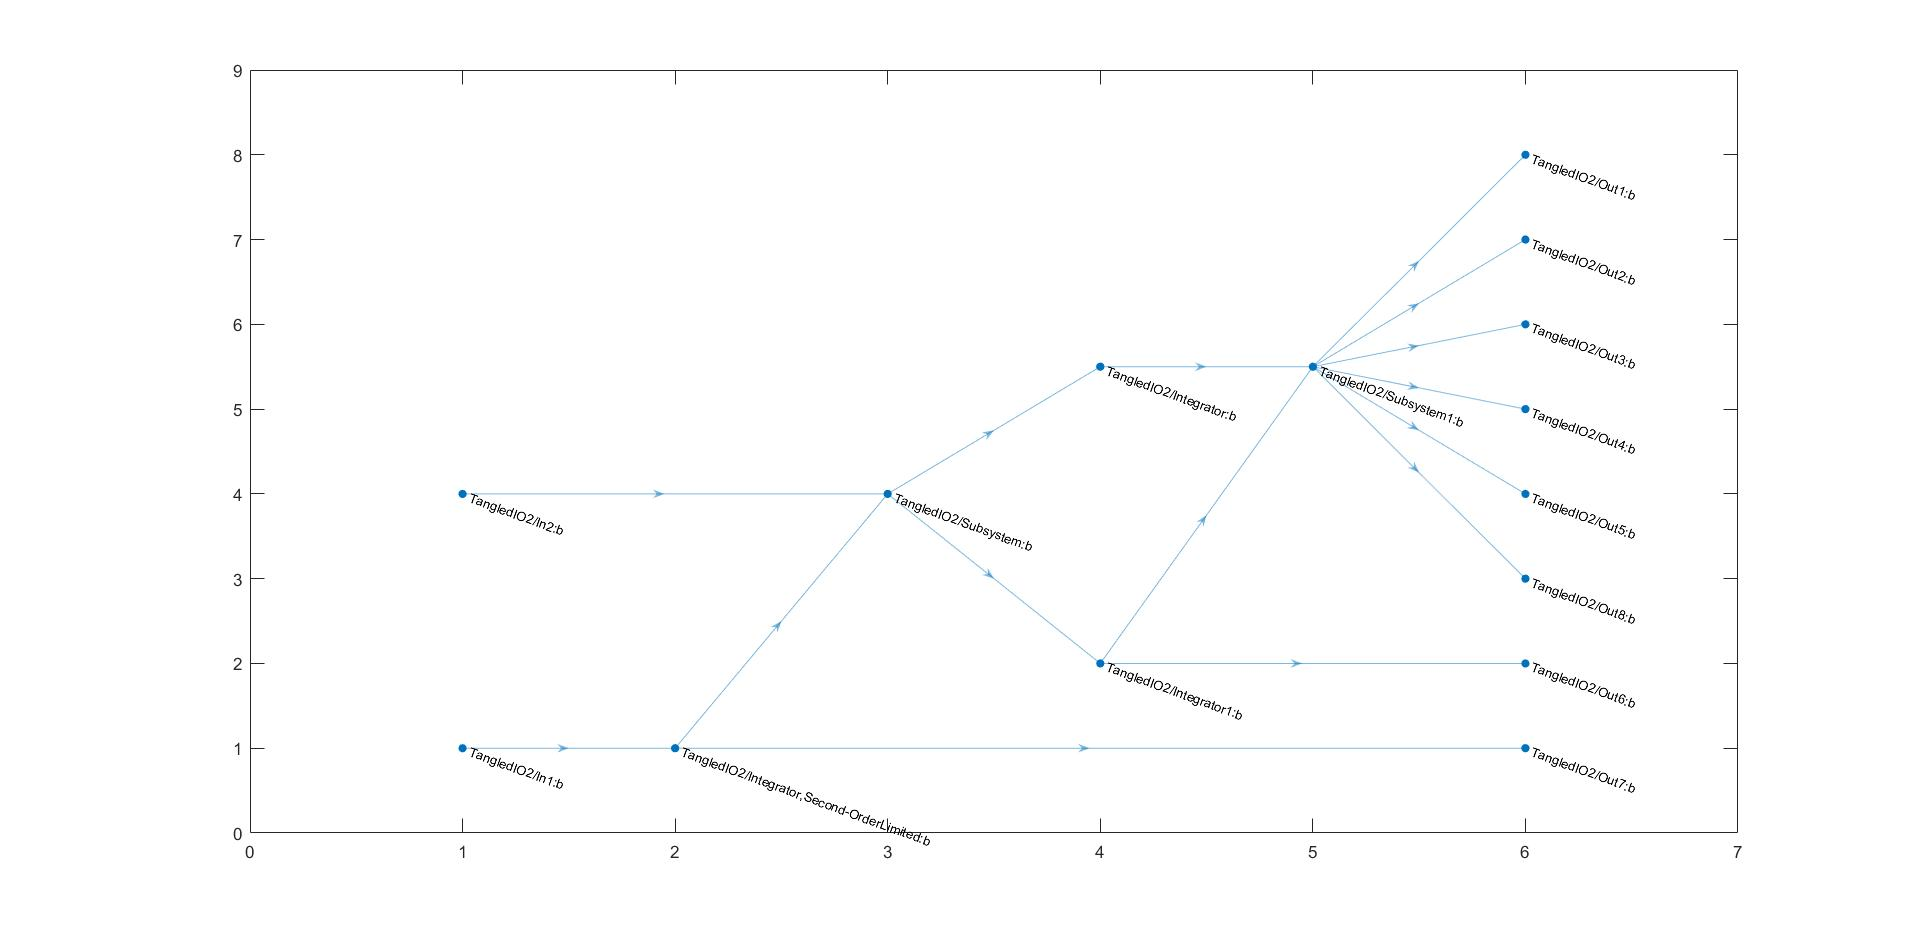
\includegraphics[width=1\linewidth]{images/graph_plot}
	\caption{GraphPlot Directed Graph Example}
	\label{fig:GraphPlotExample}
\end{figure}

\section{Hierarchy}
\par The function GraphPlotLayout is called by AutoLayout, and it calls other functions pertaining to the creation of the directed graph which represents the layout of the model. There are several modules that GraphPlotLayout calls which have similar functionality. The modules are: Arranging  Blocks, Implicit Connections, and Directed Graph. The Arranging Blocks module deals with the re-positioning of the blocks in the Simulink model. The Implicit Connections module deals with finding implicit connections in the Simulink model so that they can be added to the directed graph. The last module is Directed Graph which deals with the creation and editing of the directed graph. The GraphPlot sub-modules are functions that the \tool tool uses to interface with the MATLAB GraphPlot engine and to modify the directed graph.

%ARRANGING BLOCKS *****************************************************************************************************************************************
\section{Arranging  Blocks}
\par This module is responsible for re-arranging and re-positioning the blocks in the model. The functions in this module are:
\begin{itemize}
	\item isBranching
	\item arrangeSources
	\item arrangeSinks
	\item setPositionAL
\end{itemize}

\subsection{isBranching}
\begin{lstlisting}
function b = isBranching(lh)
% ISBRANCHING Determines if given line is a branching line.
%
%   Input:
%       lh  Line handle
%
%   Output:
%       b   Logical. True if line is branching, else false.
\end{lstlisting}
\paragraph{Internal Design:} The line is determined to be branching if it is connected to two more inputs.

\subsection{arrangeSources}
\begin{lstlisting}
function [srcs, srcPositions, didMove] = arrangeSources(blk, doMove)
% ARRANGESOURCES Finds sources of a block and swaps their vertical positions to
%   be ordered with respect to ports.
%
%   If there are branches or if a source has multiple outports, then no arranging
%   will be attempted, but positions to rearrange them will still be given as output.
%
%   Inputs:
%       blk     Simulink block fullname or handle.
%       doMove  Whether to move the blocks (1) or not (0).
%               If not, position information required to do the move is still returned.
%
%   Outputs:
%       srcs            Cell array of source block name.
%       srcPositions    Array of positions to move the srcs to.
%       didMove         Whether the blocks were moved (1) or not (0).
%                       Note: If doMove is false, didMove will always be false.
%                       If doMove is true, didMove may still be false as a
%                       result of branches/excessive ports (described above).
%
% Assumes blocks use the tradional block rotation, with inports on the left,
% and outports on the right.
\end{lstlisting}
\paragraph{Internal Design:} Rearrange the sources with respect to the input port locations of a block unless the input line branches. If the input line branches, the source block is not moved.

\subsection{arrangeSinks}
\begin{lstlisting}
function [snks, snkPositions, didMove] = arrangeSinks(blk, doMove)
% ARRANGESINKS Find the sinks of a block and swap their vertical positions to
%   be ordered with respect to ports.
%
%   If there are branches or if a sink has multiple inports, then no arranging
%   will be attempted, but positions to rearrange them will still be given as output.
%
%   Inputs:
%       blk     Simulink block fullname or handle.
%       doMove  Whether to move the blocks (1) or not (0).
%               If not, position information required to do the move is still returned.
%
%   Outputs:
%       snks            Cell array of source block name. If a line is branched,
%                       only one of those snks will be returned.
%       snkPositions    Array of positions to move the srcs to.
%       didMove         Whether the blocks were moved (1) or not (0).
%                       Note: If doMove is false, didMove will always be false.
%                       If doMove is true, didMove may still be false as a result
%                       of branches/excessive ports (described above).
%
% Assumes blocks use the tradional block rotation, with inports on the left,
% and outports on the right.
\end{lstlisting}
\paragraph{Internal Design:} Rearrange the sinks with respect to the output port locations of a block unless the output line branches. If the output line branches, the sink is not moved.

\subsection{setPositionAL}
\begin{lstlisting}
function pos = setPositionAL(block, pos)
% SETPOSITIONAL Set block position. Use this function when setting positions in
%   AutoLayout in case we want to change this in some way later.
%
%   Inputs:
%       block   Block for which to change position.
%       pos     Position to set the block to.
%
%   Outputs:
%       pos     New position of the block.
\end{lstlisting}
\paragraph{Internal Design:} The blocks are repositioned by changing their position parameter values.

%IMPLICIT CONNECTIONS ****************************************************************************************************************************************
\section{Implicit Connections}
\par This module is responsible for implicit connections (data store elements and Goto and from tags) throughout the model. The functions in this module are:
\begin{itemize}
	\item findReadWritesInScope
	\item findDataStoreMemory
	\item findVisibilityTag
	\item findGotoFromsInScope
	\item findWritesInScope
	\item findReadsInScope
	\item findGotosInScope
	\item findFromsInScope
\end{itemize}

\subsection{findReadWritesInScope} \label{findReadWritesInScope}
\begin{lstlisting}
function blockList = findReadWritesInScope(block)
% FINDREADWRITESINSCOPE Find all the Data Store Read and Data Store Write
%   blocks associated with a Data Store Memory block.
%
%   Inputs:
%       block       Data Store Memory block path name.
%
%   Outputs:
%       blockList   Data Store Read and/or Data Store Write block path names.
\end{lstlisting}
\paragraph{Internal Design:} A list of the corresponding DSR and DSW blocks are found by looking for DSR and DSW blocks that are in the scope of the DSM that also have the same variable name. Additionally, shadowing DSR and DSW blocks are ignored from the list of DSR and DSW blocks found previously by finding shadowing DSM blocks and looking for all DSR and DSW within the scope of the shadowing DSM blocks.

\subsection{findDataStoreMemory}
\begin{lstlisting}
function mem = findDataStoreMemory(block)
% FINDDATASTOREMEMORY Find the Data Store Memory block of a Data Store Read or
%   Write block.
%
%   Inputs:
%       block   Data Store Read or Write path name.
%
%   Outputs:
%       mem     Data Store Memory block path name.
\end{lstlisting}
\paragraph{Internal Design:} The corresponding DSM block is found by finding all DSM blocks with the same variable name that also contain the input block in their scope. Then, the DSM block that is closest to the input block in the model hierarchy is determined to be the corresponding DSM block.

\subsection{findWritesInScope} \label{findWritesInScope}
\begin{lstlisting}
function writes = findWritesInScope(block)
% FINDWRITESINSCOPE Find all the Data Store Writes associated with a Data
%   Store Read block.
%
%   Inputs:
%       block   Data Store Read block path name.
%
%   Outputs:
%       reads   Data Store Write block path names.
\end{lstlisting}
\paragraph{Internal Design:} The corresponding DSW block is found by finding all DSR and DSW blocks that have the same corresponding DSM block as the input DSR block. This is accomplished by using the function \hyperref[findReadWritesInScope]{findReadWritesInScope}. Then, only the DSW blocks are kept.

\subsection{findReadsInScope} \label{findReadsInScope}
\begin{lstlisting}
function reads = findReadsInScope(block)
% FINDREADSINSCOPE Find all the Data Store Read blocks associated with a Data
%   Store Write block.
%
%   Inputs:
%       block   Data Store Write block path name.
%
%   Outputs:
%       reads   Data Store Read block path names.
\end{lstlisting}
\paragraph{Internal Design:} The corresponding DSW block is found by finding all DSR and DSW blocks that have the same corresponding DSM block as the input DSR block. This is accomplished by using the function \hyperref[findReadWritesInScope]{findReadWritesInScope}. Then, only the DSR blocks are kept.

\subsection{findVisibilityTag} \label{findVisibilityTag}
\begin{lstlisting}
function visBlock = findVisibilityTag(block)
% FINDVISIBILITYTAG Find the Goto Visibility Tag block associated with a
%   scoped Goto or From block.
%
%   Inputs:
%       block     Scoped Goto or From block path name.
%
%   Outputs:
%       visBlock  Goto Tag Visibility block path name.
\end{lstlisting}
\paragraph{Internal Design:} The corresponding GTV block is found by finding all GTV blocks with the same tag name that also contain the input tag in their scope. Then, the GTV that is closest to the input block in the model hierarchy is determined to be the corresponding GTV block.

\subsection{findGotoFromsInScope}
\begin{lstlisting}
function blockList = findGotoFromsInScope(block)
% FINDGOTOFROMSINSCOPE Find all Goto and From blocks associated with a
%   Goto Tag Visibility block.
%
%   Inputs:
%       block       Goto Tag Visibility path name.
%
%   Outputs:
%       blockList   Goto and/or From block path names.
\end{lstlisting}
\paragraph{Internal Design:} A list of the corresponding GTs and FTs are found by looking for GTs and FTs that in the same scope as the GTV that also have the same variable name. Additionally, shadowing GTs and FTs blocks are ignored from the previous list by finding shadowing GTV blocks and looking for all GTs and FTs within the scope of the shadowing GTV blocks.

\subsection{findGotosInScope} \label{findGotosInScope}
\begin{lstlisting}
function goto = findGotosInScope(block)
% FINDGOTOSINSCOPE Find the Goto block associated with a From block.
%
%   Inputs:
%       block   From block path name.
%
%   Outputs:
%       goto   Goto block path name.
\end{lstlisting}
\paragraph{Internal Design:} The corresponding GT is found by first searching for a local GT. If a local GT is not found, the corresponding GTV block is searched for using the function \hyperref[findVisibilityTag]{findVisibilityTag} to determine if the GT is scoped. If a corresponding GTV is not found, then the global GT is searched for. If a corresponding GTV is found, the scoped GT and FTs corresponding to the GTV are found using the function \hyperref[findReadWritesInScope]{findReadWritesInScope}. Then, only the GT is kept.

\subsection{findFromsInScope} \label{findFromsInScope}
\begin{lstlisting}
function froms = findFromsInScope(block)
% FINDFROMSINSCOPE Find all From blocks associated with a Goto block.
%
%   Inputs:
%       block   Goto block path name.
%
%   Outputs:
%       froms   From block path names.
\end{lstlisting}
\paragraph{Internal Design:} The corresponding FTs are found by determining the scope of the input GT. If the GT is locally scoped, then the corresponding local FTs are found. If the GT is scoped, then its corresponding GTV is found using the function \hyperref[findVisibilityTag]{findVisibilityTag}, which is then used to find all FTs and the GT associated with the GTV. Lastly, if the GT is globally scoped, the corresponding FTs are found by selecting FTs from the entire model that are not scoped or local to the GT.


%DIRECTED GRAPH ****************************************************************************************************************************************
\section{Directed Graph}
\par This module is responsible for the creating and editing of the directed graph which represents the connections of the various block at a particular system level. The functions in this module are:
\begin{itemize}
	\item applyNamingConvention
	\item isdigraph
	\item plotSimulinkDigraph
	\item systemToDigraph
	\item addImplicitEdges
\end{itemize}

\subsection{applyNamingConvention}
\begin{lstlisting}
function name = applyNamingConvention(handle)
% APPLYNAMINGCONVENTION Apply a naming convention to blocks and ports.
%   May be expanded to other elements in the future.
%
%   Inputs:
%       handle  Handle of the block/port. Block name is also accepted.
%
%   Outputs:
%       name    Name with convention applied to it.
\end{lstlisting}
\paragraph{Internal Design:} Apply a naming convention to the nodes for blocks and ports. The string ":b" is appended to the names of block nodes, the string ":i" is appended to the name of inports nodes, and ":o" is appended to the name of outport nodes.

\subsection{isdigraph}
\begin{lstlisting}
function tf = isdigraph(d)
% ISDIGRAPH Return true (1) if d is a digraph and false (0) otherwise.
\end{lstlisting}
\paragraph{Internal Design:} Check if the input is a digraph.

\subsection{plotSimulinkDigraph}
\begin{lstlisting}
function h = plotSimulinkDigraph(sys, dg)
% PLOTSIMULINKDIGRAPH Plot a digraph representing a Simulink (sub)system in the
%   same fashion as a Simulink diagram, i.e., layered, left-to-right, etc.
%
%   Inputs:
%       sys     Path of the system that the digraph represents.
%       dg      Digraph representation of the system sys.
%
%   Outputs:
%       h       GraphPlot object (see
%               www.mathworks.com/help/matlab/ref/graphplot.html)
\end{lstlisting}
\paragraph{Internal Design:} Creates a GraphPlot for the digraph using the MATLAB function \textit{plot()} and specifies settings to obtain a left-to-right plot to resemble a traditional Simulink model layout. The settings used can be found here:\url{https://www.mathworks.com/help/matlab/ref/graph.plot.html}.

\subsection{systemToDigraph}
\begin{lstlisting}
function dg  = systemToDigraph(sys)
% SYSTEMTODIGRAPH Create a digraph out of the subsystem. Takes Simulink blocks
%   as nodes and their singal line connections as edges. Weights are the
%   default 1.
%
%   Inputs:
%       sys     Path of the system.
%
%   Outputs:
%       dg      Digraph representing the system.
\end{lstlisting}
\paragraph{Internal Design:} All blocks in the layout are added to the digraph as nodes. The nodes on the digraph are connected to each other using edges (lines) to represent the connections between the blocks and ports. Connections are represented by a square adjacency matrix. Connections between blocks are found by looking for what the outputs of each block in the model is connected to using each blocks connectivity parameters.

\subsection{addImplicitEdges}
\begin{lstlisting}
function dgNew = addImplicitEdges(sys, dg)
% ADDIMPLICITEDGES Add edges to a digraph representing the implicit connections
%    between goto/froms.
%
%   Inputs:
%       sys     Path of the system that the digraph represents.
%       dg      Digraph representation of the system sys.
%
%   Outputs:
%       dgNew   Updated digraph.
\end{lstlisting}
\paragraph{Internal Design:} Find all implicit connections using the functions \hyperref[findWritesInScope]{findWritesInScope}, \hyperref[findReadsInScope]{findReadsInScope}, \hyperref[findGotosInScope]{findGotosInScope}, and \hyperref[findFromsInScope]{findFromsInScope}. Then add all implicit connections to the digraph if have not been included. The connections are added to the digraph using the MATLAB function \textit{addedge()}.

\clearpage

\appendix
\chapter{List of Abbreviations} \label{A}
\begin{itemize}
	\item DSM: Data Store Memory
	\item DSW: Data Store Write
	\item DSR: Data Store Read
	\item GT: Goto Tag
	\item FT: From Tag
	\item GVT: Goto Visibility Tag
\end{itemize}

\end{document}